\chapter{Bifurcation}

\section{Introduction}

Consider a nice function $f:\RR^2 \rightarrow \RR$.  It defines a
one-parameter family of functions $f_\mu(x) = f(x,\mu)$.

We say that $\mu = \mu_0$ is a bifurcation point of the discrete
dynamical system\index{Bifurcation point}
\[
x_{i+1} = f_\mu(x_i)
\]
if the qualitative behaviour of the {\bfseries phase portrait} (the
plot on the real line of the orbits under $f_\mu$) changes as $\mu$
goes through $\mu_0$.  For instance, new periodic solutions appear,
etc.\nomenclature{$\mu$}{Bifurcation parameter}

There are three major results related to bifurcation.  The first
result is a simple consequence of the Implicit Function Theorem.

\begin{theo} \label{IFTforDS}
Let $f:\RR^2 \rightarrow \RR$ be a smooth function and let
$f_\mu(x)= f(x,\mu)$.  Suppose that $f_{\mu_0}(x_0) = x_0$ and
\[
\frac{\partial}{\partial x} f_{\mu}(x)\bigg|_{\mu=\mu_0,x=x_0} \neq 1  \ ,
\]
then there exist an interval $I$ about $x_0$, an interval $U$ about
$\mu_0$, and a mapping $p:U\rightarrow I$ such that $p(\mu_0)=x_0$ and
$f_\mu(p(\mu))=p(\mu)$ for all $\mu \in U$.  Moreover, $f_\mu$ has no
other fixed point in $I$.
\end{theo}

The next theorems describe two important types of bifurcation.

\begin{theo}[Saddle-Node]
Let $f:\RR^2 \rightarrow \RR$ be a smooth function and let
$f_\mu(x)= f(x,\mu)$.  Suppose that
\begin{enumerate}
\item $\displaystyle f_{\mu_0}(0)=0$,
\item $\displaystyle \frac{\partial}{\partial x}
f_{\mu}(x)\bigg|_{\mu=\mu_0,x=0} = 1$,
\item $\displaystyle \frac{\partial^2}{\partial x^2}
f_{\mu}(x)\bigg|_{\mu=\mu_0,x=0} \neq 0$, and
\item $\displaystyle \frac{\partial}{\partial \mu}
f_\mu(x)\big|_{\mu=\mu_0,x=0} \neq 0$.
\end{enumerate}
Then, there exist an interval $I$ about $0$ and a mapping
$q:I\rightarrow \RR$ such that $f_{q(x)}(x) = x$.  Moreover,
$q'(0) = 0$ and $q''(0) \neq 0$.
\end{theo}

\begin{theo}[Period Doubling]
Let $f:\RR^2 \rightarrow \RR$ be a smooth function and let
$f_\mu(x)= f(x,\mu)$.  Suppose that
\begin{enumerate}
\item $f_{\mu}(0)=0$ for all $\mu$ near $\mu_0$,
\item $\displaystyle \frac{\partial}{\partial x}
f_{\mu}(x)\bigg|_{\mu=\mu_0,x=0} = -1$,
and
\item $\displaystyle \frac{\partial^2}{\partial x \partial \mu}
f_{\mu}^2(x)\bigg|_{\mu=\mu_0,x=0} \not=0$
\end{enumerate}
(note that $f^2_\mu(x) \equiv f(f(x,\mu),\mu)$\ ).  Then, there exist
an interval $I$ about $0$ and a mapping $q:I\rightarrow \RR$ such that
$f_{q(x)}(x) \neq x$ but $f^2_{q(x)}(x) = x$.
\end{theo}

\begin{egg}
For the logistic map $f_\mu(x) = \mu x(1-x)$, there is period doubling
at $\mu=3$.  We have
$f_\mu(p_\mu) = p_\mu$ for all $\mu$ near $\mu=3$,
$\displaystyle \frac{\partial}{\partial x} f_3(p_3) = -1$ and
\begin{align*}
\frac{\partial^2}{\partial \mu \partial x} f_\mu^2(x) \big|_{\mu=3,x=p_\mu} &=
\left( 2\mu - 6\mu^2 x+18\mu^2 x^2 - 4\mu x -
12\mu^2 x^3\right)\big|_{\mu=3,x=p_\mu} \\
&= -2 \not=0
\end{align*}
\end{egg}

\section{More examples of \LaTeX}

Here is an example of a footnote\footnote{This section just illustrates
some features of \LaTeX}

\begin{table}
\begin{tabular}{c|c|l}
\cline{1-3}
$b$ & $C_b$ & Commentaires \\ 
\cline{1-3}
$2.0$ & $0.69314718409\ldots$ & \\ 
$2.1$ & $0.74193735600\ldots$ & \\ 
$2.2$ & $0.78845736606\ldots$ & \\ 
 \vdots & \vdots & \vdots \\
$2.7$ & $0.99325176972\ldots$ & \\ 
$2.8$ & $1.02961941195\ldots$ &
     $C_b$ est sup\'erieure \`a $1$, on retourne \\
 & & \`a la valeur de $b$ pr\'ec\'edente (i.e. $2.7$) \\
 & & et continue en ajoutant $10^{-2}$. \\
$2.71$ & $0.99694863476\ldots$ & \\ 
$2.72$ & $1.00063188846\ldots$ &
     $C_b$ est sup\'erieure \`a $1$, on retourne \\
 & & \`a la valeur de $b$ pr\'ec\'edente (i.e. $2.71$) \\
 & & et continue en ajoutant $10^{-3}$. \\
$2.711$ & $0.99731758407\ldots$ & \\ 
$2.712$ & $0.99768637796\ldots$ & \\ 
 \vdots & \vdots & \vdots \\
$2.718$ & $0.99989632130\ldots$ & \\ 
$2.719$ & $1.00026416039\ldots$ &
     $C_b$ est sup\'erieure \`a $1$, on retourne \\
 & & \`a la valeur de $b$ pr\'ec\'edente (i.e. $2.718$) \\
 & & et continue en ajoutant $10^{-4}$. \\
$2.7181$ & $0.99993311409\ldots$ & \\ 
$2.7182$ & $0.99996990688\ldots$ & \\ 
 \vdots & \vdots & \vdots \\
$2.71828182852$ & $0.99999999392253\ldots$ & \\ 
\cline{1-3}
\end{tabular}
\caption[Une approximation de $e$]{Une approximation de $e$ \label{TAB_EXP}}
\end{table}

On retrouve au Tableau~\ref{TAB_EXP}, une approximation du nombre $b$
tel que
\begin{equation} \label{COND_EXP}
C_b \equiv \lim_{h\rightarrow 0} \frac{b^h-1}{h} = 1
\end{equation}

\newpage

\begin{figure}
\begin{center}
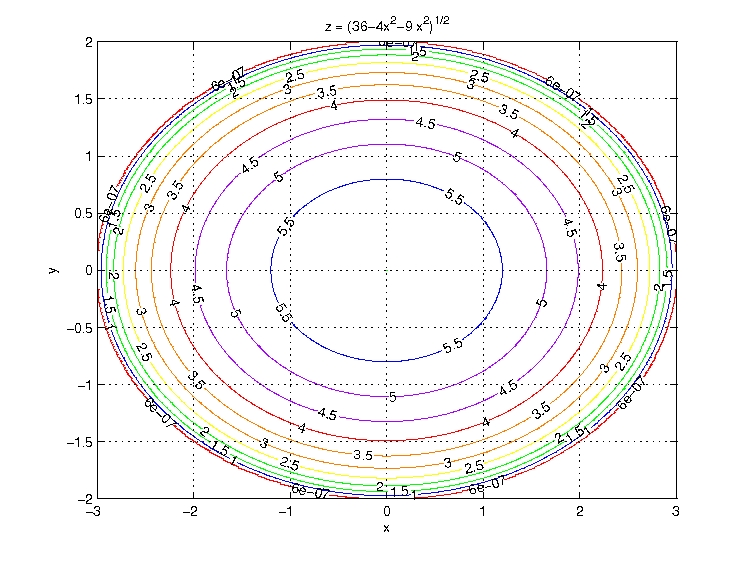
\includegraphics[width=10cm]{lev_curves1}
\end{center}
\caption[A short description for the list of tables]{Quelques courbes de
  niveau pour la fonction $f(x,y) = \sqrt{36-4x^2-9y^2}$.  On obtient
  des ellipses.  This is a very long long long long long long long
  long long long long long long long long long long long long long
  long long long long long long long description for a figure.
  \label{LEV_CURV1}}
\end{figure}

\begin{figure}
\begin{center}
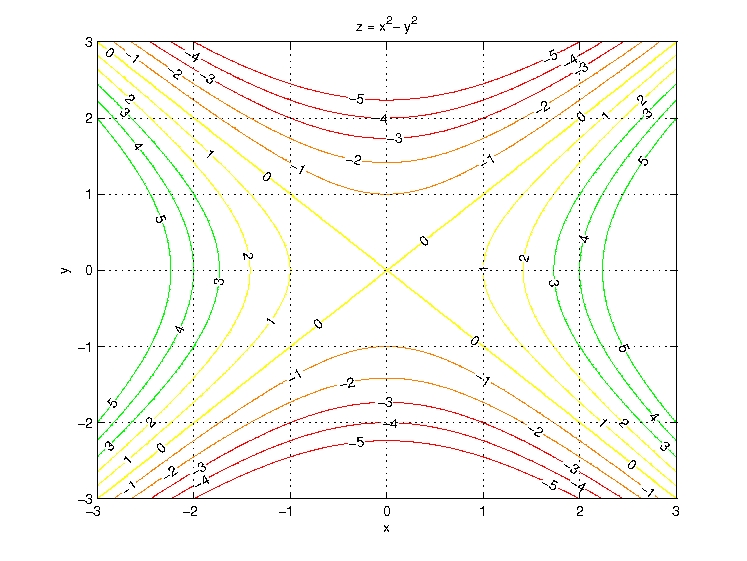
\includegraphics[width=10cm]{lev_curves2}
\end{center}
\caption[Courbes de niveau pour $f(x,y) = x^2-y^2$]{Quelques courbes de
  niveau pour la fonction $f(x,y) = x^2-y^2$.  On obtient des hyperboles.
  \label{LEV_CURV2}}
\end{figure}

\begin{figure}
\begin{center}
\setlength{\unitlength}{1.00 cm}
\begin{picture}(1,5)(2,-0.5)
\put(0,0){\vector(1,0){8}}
\put(0,0){\vector(0,1){4}}
\put(-0.5,4){$y$}
\put(8,-0.5){$x$}
\qbezier(-1,1)(3,5)(6,-2)
\put(4.8,-0.5){$p$}
\put(3.35,-0.5){$x_n$}
\multiput(3.5,0.0)(0,0.2){9}{\line(0,1){0.1}}
\put(6,-0.5){$x_{n+1}$}
\put(2.3,2.7){\line(4,-3){3.55}}
\put(2,3){$y=f(x)$}
\put(4,2){tangent line at $(x_n,f(x_n))$}
\end{picture}
\end{center}
\caption[Newton-Raphson]{Newton-Raphson \label{NRM}}
\end{figure}

This table has nothing to do with discrete dynamical systems.  It
illustrates the use of the environment tabular.

\begin{center}
\begin{tabular}{|c|c|c|}
\hline
$x$ & \multicolumn{2}{|c|}{values} \\
\hline
$1$ & $\displaystyle \int_0^6 \, \ln(1+x^2)\,\text{d}x$ & $0$ \\
\cline{1-1}
\multicolumn{2}{|c|}{This is modern Arts} & $2$ \\
\hline
\end{tabular}
\end{center}

Same story for the next table.  However, this time, the figure
illustrates the use of the environment array in math. mode.

\[
\begin{array}{|c|c|c|}
\hline
x & \multicolumn{2}{|c|}{\text{values}} \\
\hline
1 & \displaystyle \int_0^6 \, \ln(1+x^2)\,\text{d}x & 0 \\
\cline{1-1}
\multicolumn{2}{|c|}{\text{This is modern Arts}} & 2 \\
\hline
\end{array}
\]

\subsection{Commutative Diagrams}

This is a simple commutative diagram that can be produced with the package
{\em amscd} which is loaded in UOthesis.sty.
\[
\begin{CD}
\ldots @>>> H_q(x) @>H_q(f)>> H_q(Y) @>>> H_q(Cf) @>>> H_{q-1}(x) @>>>
\ldots\\
@.  @V{H_q(\alpha)}VV  @VH_q(\beta)VV  @VH_q(\gamma)VV  @VH_{q-1}(\alpha)VV 
@. \\
\ldots @>>> H_q(X') @>>H_q(f')> H_q(Y') @>>> H_q(Cf') @>>> H_{q-1}(X') @>>>
\ldots
\end{CD}
\]
For those graduate students who want to upset their supervisor (at their own
risk), they could instead produce the following commutative diagram.
\[
\begin{CD}
\ldots @<<< H_{q-1}(X') @<<< H_q(Cf') @<<< H_q(Y') @<H_q(f')<< H_q(X') @<<<
\ldots \\
@.  @AAH_{q-1}(\alpha)A  @AAH_q(\gamma)A  @AAH_q(\beta)A  @AA{H_q(\alpha)}A 
@. \\
\ldots @<<< H_{q-1}(x) @<<< H_q(Cf) @<<< H_q(Y) @<<H_q(f)< H_q(x) @<<<
\ldots\\
\end{CD}
\]

However, the package {\em amscd} is limited.  The following commutative
diagram associated to the first isomorphism theorem has been produced with
the picture environment.
\begin{center}
\setlength{\unitlength}{1.5em}
\begin{picture}(4,3)
\put(0,2){$G$}              % (0,0) is the lower left corner
\put(3,2){$\IM f$}
\put(0,0){$G/\KER f$}
\put(1,2.2){\vector(1,0){1.8}}
\put(1.8,2.4){\scriptsize $f$}
\put(0.2,1.8){\vector(0,-1){1}}
\put(-0.25,1.25){\scriptsize $\pi$}
\put(1,0.8){\vector(3,2){1.6}}
\put(2.2,1.1){\scriptsize $f$}
\end{picture}
\end{center}
where $f:G\rightarrow H$ is a group homomorphism.  The result is good but
it took a long time to fix the different positions and lengths to get the
diagram above.  It is probably not the fastest way to produce commutative
diagrams.

One can also use drawing programs like {\bfseries xfig} to produce
commutative diagrams but the results may not be terrific and some time has to
be spent to learn how to use a drawing program.

The serious alternative is the package {\em xy} (i.e. the
$\text{X}_\text{\normalsize Y}$-pic code).  It is easy to use (if one sticks
to the basic) and one can draw any imaginable diagrams (including commutative
diagrams).  The package {\em xy} is not loaded by the style file
UOthesis.sty.  So, one has to load it in the file template.tex (or whatever
the name one gives to it) with the command \verb=\usepackage[all]{xy}= as it
is done in the present example. Using this package, the previous commutative
diagram for the first isomorphism theorem becomes
\[
\xymatrix{
G \ar[r]^f \ar[d]_{\pi} & \IM f \\
G/\KER f \ar[ur]_{f} &
}
\]
The code
\begin{verbatim}
\[
\xymatrix{
G \ar[r]^f \ar[d]^{\pi} & \IM f \\
G/\KER f \ar[ur]_{f}  &
}
\]
\end{verbatim}
needs to be explained.  The command \verb=\ar[]= creates an arrow from the
cell where the command is used to the cell specified inside the square
brackets.  A logical combination of the following letters can be used inside
the square brackets: r = cell to the right, l = cell to the left, u = cell
above, d = cell below.  The arguments provided by \verb=^{}= or \verb=_{}= to
\verb=\ar[]= are written to the left or right of the arrow if looking
forward.

Obviously, you may modify the arrows to produce some non-sense.
\[
\xymatrix{
G \ar@{-->}[r]^f \ar@{|=>}[d]_{\pi} & \IM f \\
G/\KER f \ar@{.>}[ur]_{f} &
}
\]
If you look at the source of this file, you will find that the command
\verb=\ar@{}[[]= has been used instead of the command \verb=\ar[]=.
The command \verb=\ar@{}[]= has the same meaning than \verb=\ar[]= above.
The option between the braces could be any logical combination of $<$, $>$,
$=$, $--$, $.$, $|$, etc.  

The following examples shows what could be done with the package {\em xy}.
\[
\begin{xy}
(0,0)*[o]+{L};(50,20)*[o]+{R}=        % L is at (0,20) and R at (40,20) ,
                                % the option [o] put the letter at the center
                                % of a circle centered at the given
                                % coordinates.  The option [o]+[F] will draw
                                % the frame of this circle.
"R"**\crv{} ? (0.4)*@{>}*^+!UL{f_1},     % line from (0,0) to (50,20) , add a
                                % + sign at 40% of the line and write f_1 under
                                % the line and to the right of the +
"R"**\crv{(30,30)} ? *@{>}*^+!DR{f_2},   % spline through (0,0), (30,30) and
                                % (50,20) , add a + at 50% of the line and
                                % write f_2 above the line and to the left of
                                % the +
"R"**\crv{(20,30)&(30,40)} ? *@{>}*^+!DR{f_3},      % spline through (0,0),
                                % (20,30), (30,40) and (50,20), add a + sign
                                % at 50% of the line and write f_3 above the
                                % line and to the left of the +
"R"**\crv{(10,-20)&(25,-20)&(35,15)} ? (0.6)*@{<}*^+!UL{f_4}   % spline
                                % through (0,0), (10,-20),(25,-20), (40,20)
                                % and (50,20) , add a + sign at 60% of the
                                % line and write f_4 below the line and to
                                % the right of the +
\end{xy}
\]

Note that the meaning of L and R are inverted, and the meaning of D and U
are also inverted.

\[
\begin{xy}
<1cm,0cm>:(0,0)*+@{*}="a"*+!DR{A}, "a"   % draw the point at the origin and
                                % write  A above and left to the origin.
\ar@(dr,dl)^{e_a}  % draw an arrow from  A to A (leave down right and come back
              % down left)
\ar@{^>}^f (2,0)*+@{*}="b"*+!DL{B}, "b"  % draw a weird arrow from  A to B, draw
                                % the point at (2,0) and write B above and
                                % right of (2,0)
\ar@(r,d)^{e_b} "b"; "b" % draw a line from  B  to itself (leave right and come
                     % back down)
\ar@{<-->}_{g} "b"; (2,2)*+@{*}="c"*+!UL{C}, "c"  % draw an bidirectional arrow
                                % from  B to C, draw the point at (2,2) and
                                % write  C below and right to (2,2)
\ar@(u,r)^{e^{-1}_c} "c"; "c"  % draw an arrow from  C  to itself (leave up
                              % and come back right)
\ar@(ul,dr)^{h} "c"; (0,2)*+@{*}="d"*+!UR{D}, "d"  % draw an arrow from  C to D,
                                % draw the point at (0,2) and write  D below
                                % and right of (0,2).  Note that the arrow
                                % leaves C up and left and arrive at D down
                                % right
\ar@(ul,ur)^{q} "d"; "d" % draw an arrow from  C  to itself (leave up left
                         % and come back up right)
\ar@{.>}^{\alpha} "d"; "a"  % draw a dotted arrow from D to A
\ar@{=>}^{\beta^{-1}} "c"; "a"  % draw a double line arrow from C to A
\end{xy}
\]

For more information on $\text{X}_\text{\normalsize Y}$-pic (including a
user guide, a reference manual, and many examples), visit the web site
\url{http://www.tug.org/applications/Xy-pic/Xy-pic.html}.

\subsection{The Picture Environment}

Figure~\ref{STFig1} is an example of the picture environment provided by one
of your colleagues.

\begin{figure}
\begin{center}
\begin{picture}(200,200)(0,-20)
% %\put(200,50){\line(1,0){100}}
% %\put(200,50){\line(0,1){50}}
% %\put(55,180){\line(1,0){100}}
% %\put(55,180){\line(0,1){120}}
\put(105,100){\line(1,0){95}}
\put(105,100){\line(0,1){100}}
% %\put(175,100){\vector(1,0){40}}
% %\put(175,100){\vector(0,1){40}}
% %\put(225,240){\vector(1,0){40}}
% %\put(225,240){\vector(0,1){40}}
% % \put(55,180){\circle{5}}
% %\put(200,50){\circle{5}}
\put(95,30){\circle*{5}}
% %\put(125,240){\circle*{5}}
\put(105,100){\circle{5}}
\put(165,120){\circle*{5}}
\put(125,140){\circle*{5}}
% %\put(80,190){\circle*{5}}
\put(115,160){\circle*{5}}
\put(130,150){\circle*{5}}
\put(40,140){\circle*{5}}
\put(180,50){\circle*{5}}
\put(170,190){\circle*{5}}
\put(190,120){\circle*{5}}
\put(70,10){\circle*{5}}
\put(140,130){\circle*{5}}
\put(175,180){\circle*{5}}
\put(20,180){\circle*{5}}
% %\put(245, 10){\circle*{5}}
\put(175,180){\circle*{5}}
\put(125,190){\circle*{5}}
% %\put(150,190){\circle*{5}}
\put(145,170){\circle*{5}}
\put(170,105){\circle*{5}}
\put(157,165){\circle*{5}}
% %\put(50,60){\Large$\tau^{(1)}$}
\put(165,145){$\bf \xi$}
% %\put(135,140){\Large$\tau^{(3)}$}
% %\put(175,150){\Large$\tau^{(1)}$}
% %\put(165,200){\Large$\tau^{(4)}$}
% %\put(215,220){\Large$\tau^{(5)}$}
% %\put(-20,-20){(0,0)}
% %\put(60,60){\vector(1,1){35}}
% %\put(60,70){\vector(1,1){30}}
% %\put(75,60){\vector(1,1){30}}
% %\put(160,10){\vector(1,1){35}}
% %\put(160,20){\vector(1,1){30}}
% %\put(170,10){\vector(1,1){30}}
% %\put(15,140){\vector(1,1){35}}
% %\put(15,150){\vector(1,1){30}}
% %%\put(25,140){\vector(1,1){30}}
\put(0,-10){{\circle*{5}} $= \sigma$, unobserved jump point of $L$}
\put(0,-20){{\circle{5}} observed points of $N$}
\put(0,0){\framebox(200,200){}}
% %\put(0,0){\circle{5}}
%\put(0,-30){\circle{5}}
\end{picture}
\end{center}
\caption{A change-set $\xi$ generated by a single point $\sigma$.
\label{STFig1}}
\end{figure}

\clearpage

\subsection{Rotating}

It is possible to rotate blocks of text, figures, ...  For instance, the
following matrix has been rotated by $90$ degrees.

\begin{sideways}
\parbox{20cm}{
\[
\left( 
\begin{array}{cccccccccccccc}
1234 & 1234 &1234 &1234 &1234 &1234 &1234 &1234 &1234 &1234 &1234 &1234 &1234
&1234 \\
2345 & 2345 &2345 &2345 &2345 &2345 &2345 &2345 &2345 &2345 &2345 &2345 &2345
&2345
\end{array}
\right)
\]
}
\end{sideways}

Similarly, Table~\ref{TTBB1} has been rotated by $90$ degrees.

\begin{table}
\begin{sideways}
\begin{tabular}{ccccc}
\multicolumn{5}{l}{a) $x_0 < x_1 <x_2 < x_3$} \\
&&&&\\
$\displaystyle x_i$ & $\displaystyle f[\cdot] $ &
$\displaystyle f[\cdot,\cdot]$ &
$\displaystyle f[\cdot,\cdot,\cdot]$ &
$\displaystyle f[\cdot,\cdot,\cdot,\cdot]$ \\
\hline
\rule{0em}{2em} $\displaystyle x_0$ & \multicolumn{1}{|c}{$\displaystyle
  f(x_0)$} &
\multicolumn{1}{|c}{$\displaystyle f[x_1,x_0] =
  \frac{f(x_1)-f(x_0)}{x_1-x_0}$} &
\multicolumn{1}{|c}{$\displaystyle
  f[x_2,x_1,x_0]=\frac{f[x_2,x_1]-f[x_1,x_0]}{x_2-x_0}$} &
\multicolumn{1}{|c|}{$\displaystyle f[x_3,x_2,x_1,x_0] =
\frac{f[x_3,x_2,x_1]-f[x_2,x_1,x_0]}{x_3-x_0}$} \\[1em]
\cline{2-5}
\rule{0em}{2em} $\displaystyle x_1$ & $\displaystyle f(x_1)$ &
$\displaystyle f[x_2,x_1] = \frac{f(x_2)-f(x_1)}{x_2-x_1}$ &
$\displaystyle f[x_3,x_2,x_1] = \frac{f[x_3,x_2]-f[x_2,x_1]}{x_3-x_1}$
& \\[1em]
\rule{0em}{2em} $\displaystyle x_2$ & $\displaystyle f(x_2)$ &
$\displaystyle f[x_3,x_2] = \frac{f(x_3)-f(x_2)}{x_3-x_2}$ & & \\[1em]
$\displaystyle x_3$ & $\displaystyle f(x_3)$ & & &
\end{tabular}
\end{sideways}
\caption{Examples of table of Newton Divided Differences\label{TTBB1}}
\end{table}

or, if you prefer to have the caption also rotated by $90$ degrees, you can
also produce Table~\ref{TTBB2}.

\begin{sidewaystable}
\hspace*{-3em}   % This may be needed to shift the table down a little
                 % because it otherwise overlaps with the header.
\begin{tabular}{ccccc}
\multicolumn{5}{l}{a) $x_0 < x_1 <x_2 < x_3$} \\
&&&&\\
$\displaystyle x_i$ & $\displaystyle f[\cdot] $ &
$\displaystyle f[\cdot,\cdot]$ &
$\displaystyle f[\cdot,\cdot,\cdot]$ &
$\displaystyle f[\cdot,\cdot,\cdot,\cdot]$ \\
\hline
\rule{0em}{2em} $\displaystyle x_0$ & \multicolumn{1}{|c}{$\displaystyle
  f(x_0)$} &
\multicolumn{1}{|c}{$\displaystyle f[x_1,x_0] =
  \frac{f(x_1)-f(x_0)}{x_1-x_0}$} &
\multicolumn{1}{|c}{$\displaystyle
  f[x_2,x_1,x_0]=\frac{f[x_2,x_1]-f[x_1,x_0]}{x_2-x_0}$} &
\multicolumn{1}{|c|}{$\displaystyle f[x_3,x_2,x_1,x_0] =
\frac{f[x_3,x_2,x_1]-f[x_2,x_1,x_0]}{x_3-x_0}$} \\[1em]
\cline{2-5}
\rule{0em}{2em} $\displaystyle x_1$ & $\displaystyle f(x_1)$ &
$\displaystyle f[x_2,x_1] = \frac{f(x_2)-f(x_1)}{x_2-x_1}$ &
$\displaystyle f[x_3,x_2,x_1] = \frac{f[x_3,x_2]-f[x_2,x_1]}{x_3-x_1}$
& \\[1em]
\rule{0em}{2em} $\displaystyle x_2$ & $\displaystyle f(x_2)$ &
$\displaystyle f[x_3,x_2] = \frac{f(x_3)-f(x_2)}{x_3-x_2}$ & & \\[1em]
$\displaystyle x_3$ & $\displaystyle f(x_3)$ & & &
\end{tabular}
\caption{Examples of table of Newton Divided Differences\label{TTBB2}}
\end{sidewaystable}

Obviously, there are many more \begin{turn}{30}
  possibilities \end{turn}.\\[2em]
It is up to you to \begin{rotate}{30} create \end{rotate} \hspace{1em}
\begin{rotate}{-30} the \end{rotate} \hspace{1em} desired effect.

\newpage

\subsection{PDF files}

We end this sample of a thesis by including a PDF files which normally
should be a research paper.

\includepdf[pages=-,noautoscale=true,scale=0.9,
pagecommand={\thispagestyle{plain}}]{MAT2331_Summary.pdf}


%%% Local Variables: 
%%% mode: latex
%%% TeX-master: "template"
%%% End: 
